\chapter{Satellite Data}
\label{Appendix: Satellite Data}
\section{Aqua Monitor Data}
In this part, one can find all the created maps for the water gains and losses from 1985-2025. 
Using the code from Deltares on Github, and adapting it to Google Earth Engine in function of the requirements from the team, one can find the following maps in Chaper \ref{chap:results}.

\begin{figure}[H]
    \centering
    % First row of subfigures
    \begin{subfigure}[b]{0.48\textwidth}
        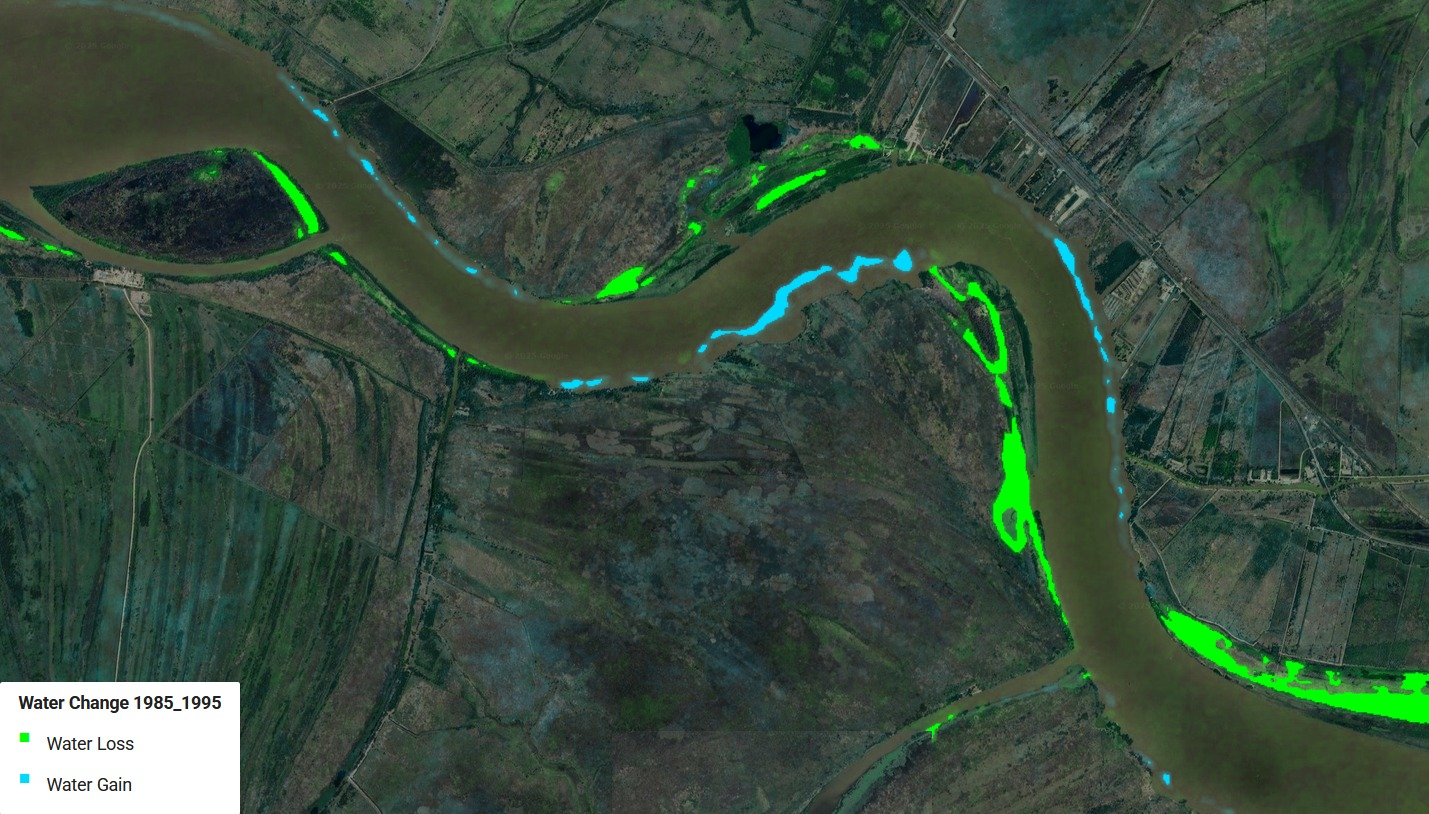
\includegraphics[width=\linewidth, height =5cm]{figures/appendix-g/1985-1995.jpg}
        \caption{1985-1995}
        \label{fig:second}
    \end{subfigure}
    \hfill
    \begin{subfigure}[b]{0.48\textwidth}
        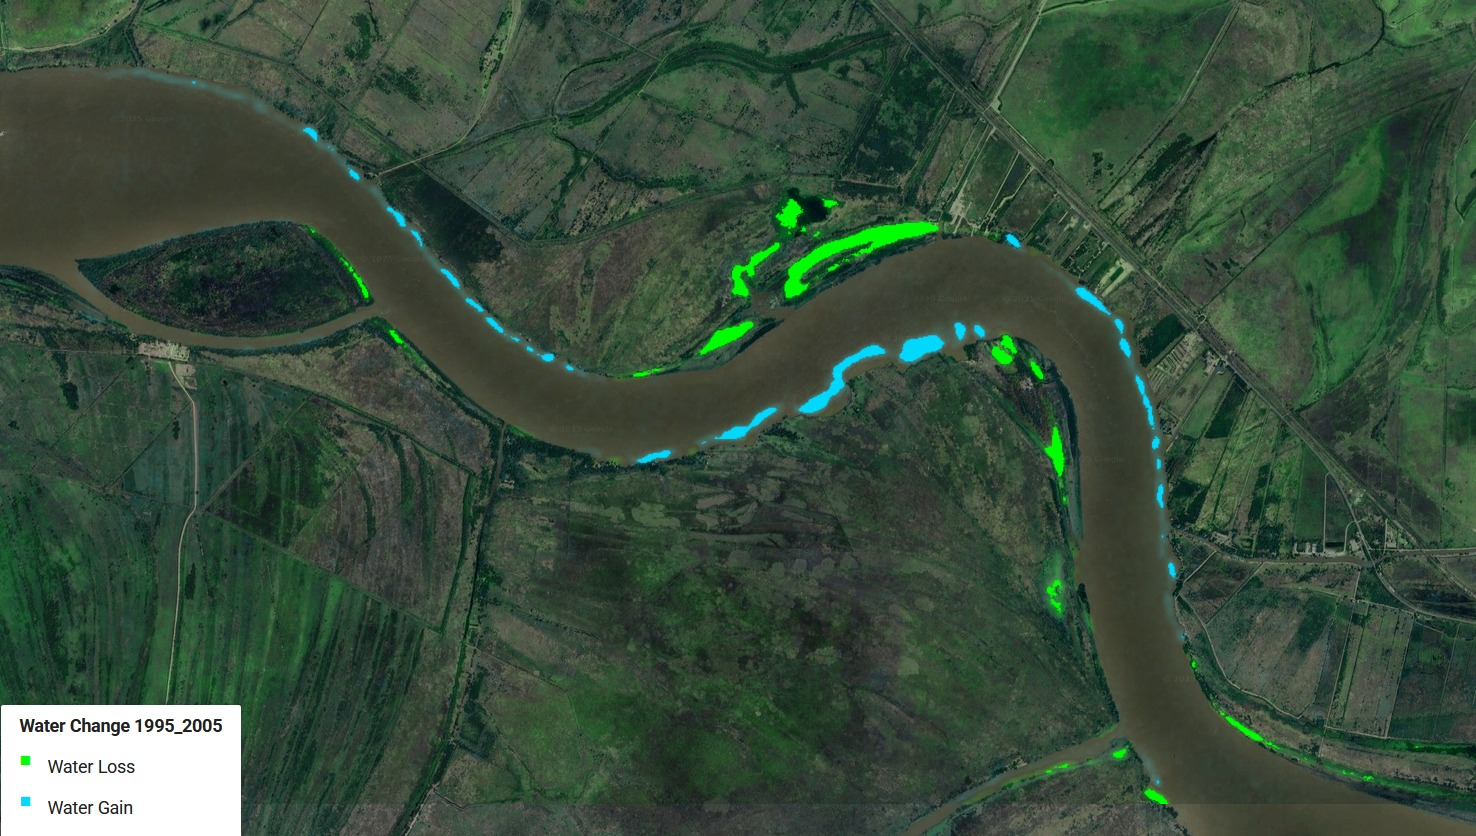
\includegraphics[width=\linewidth, height =5cm]{figures/appendix-g/1995-2005.jpg}
        \caption{1995-2005}
        \label{fig:second}
    \end{subfigure}
    

    % Second row of subfigures (add some vertical space)
    \vspace{0.5cm}

    % Second row of subfigures
    \begin{subfigure}[b]{0.48\textwidth}
        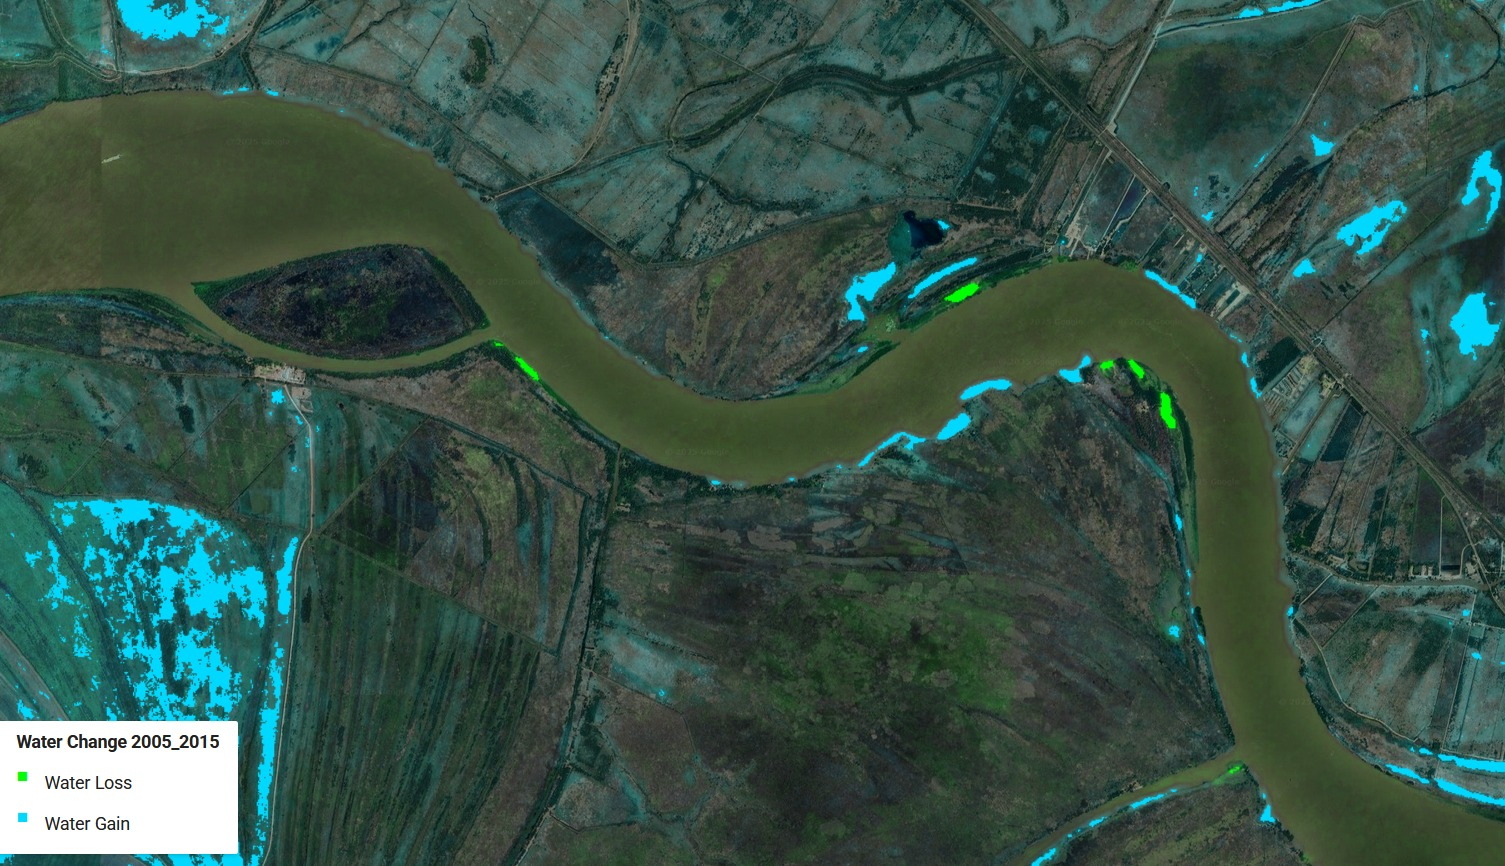
\includegraphics[width=\linewidth, height =5cm]{figures/appendix-g/2005-2015.jpg}
        \caption{2005-2015}
        \label{fig:second}
    \end{subfigure}
    \hfill
    \begin{subfigure}[b]{0.48\textwidth}
        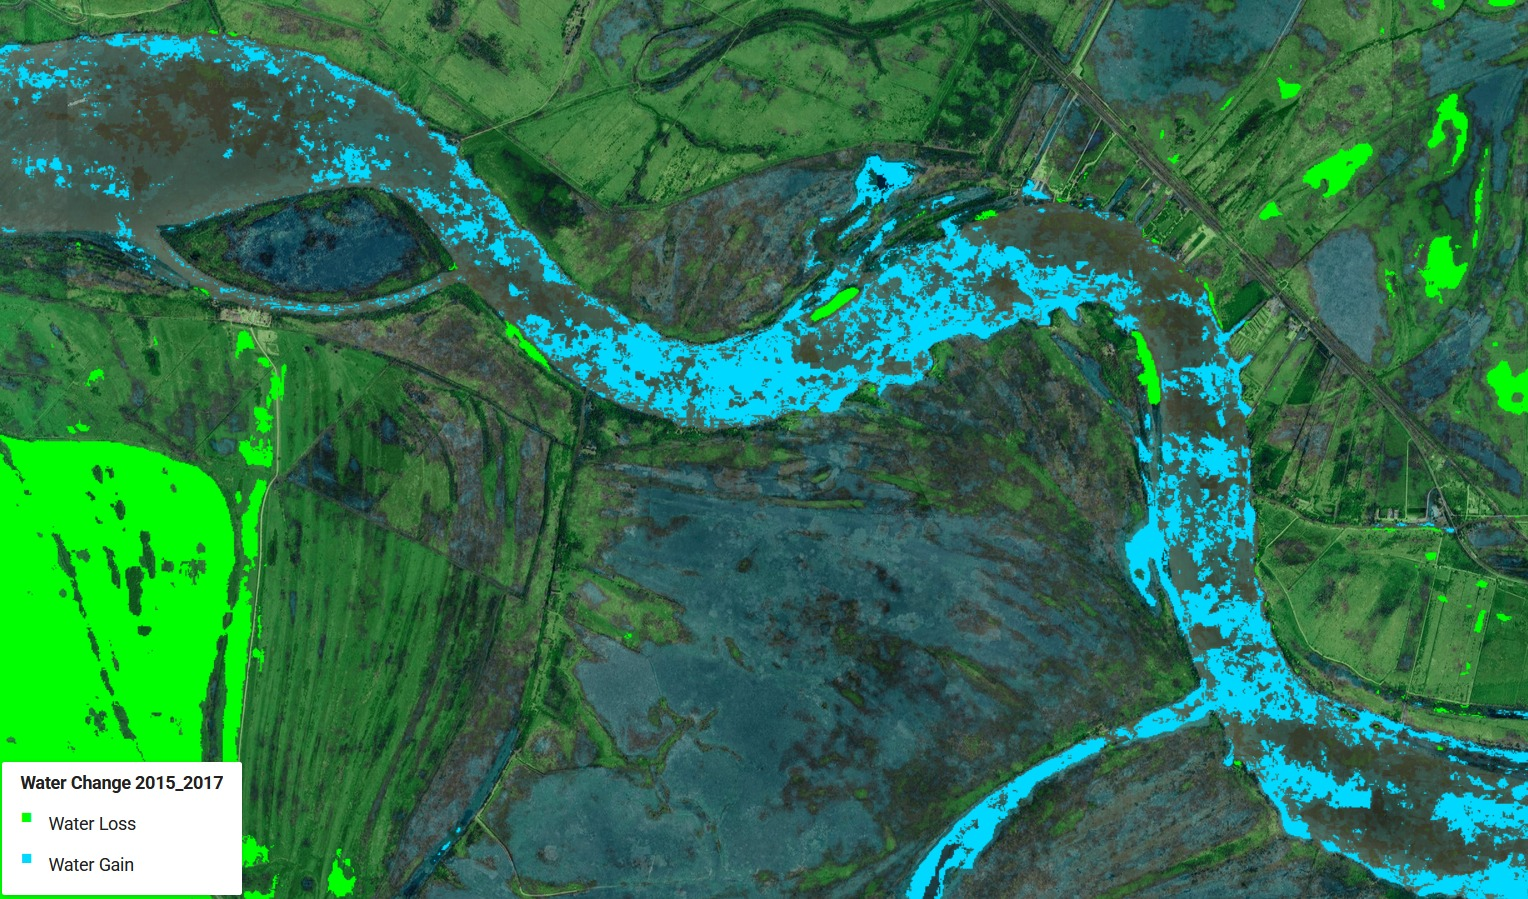
\includegraphics[width=\linewidth, height =5cm]{figures/ch5/2015-2017.jpg}
        \caption{2015-2017}
        \label{fig:second}
    \end{subfigure}

    \caption{All Changes in Water on the Area of Interest Part 1}
    \label{fig:All Changes in Water on the Area of Interest Part 1}
\end{figure}

\begin{figure}[H]
    \centering
    % First row of subfigures
    \begin{subfigure}[b]{0.48\textwidth}
        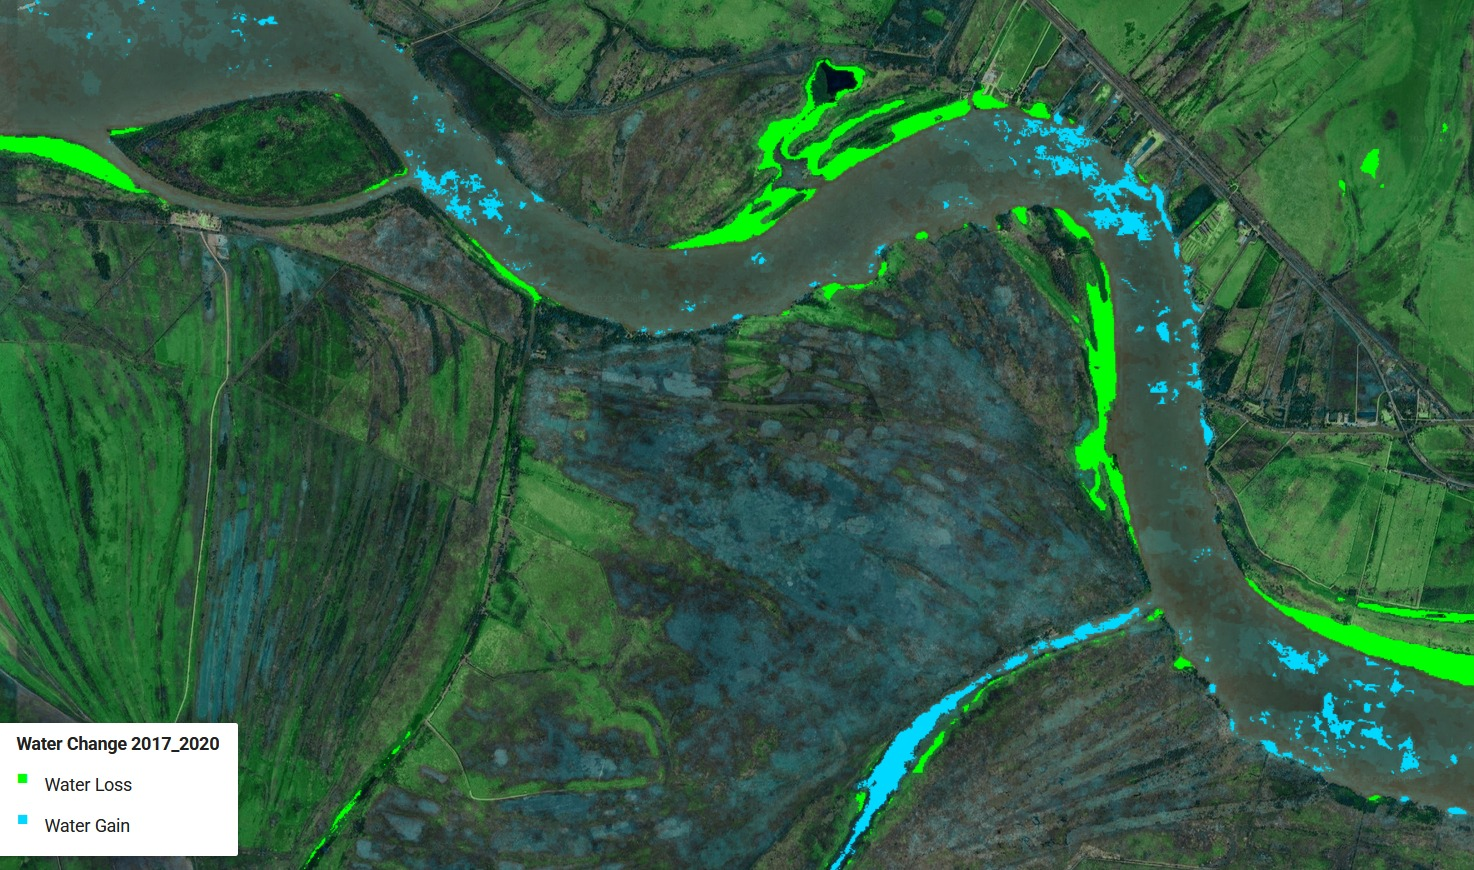
\includegraphics[width=\linewidth, height =5cm]{figures/appendix-g/2017-2020.jpg}
        \caption{2017-2020}
        \label{fig:second}
    \end{subfigure}
    \hfill
    \begin{subfigure}[b]{0.48\textwidth}
        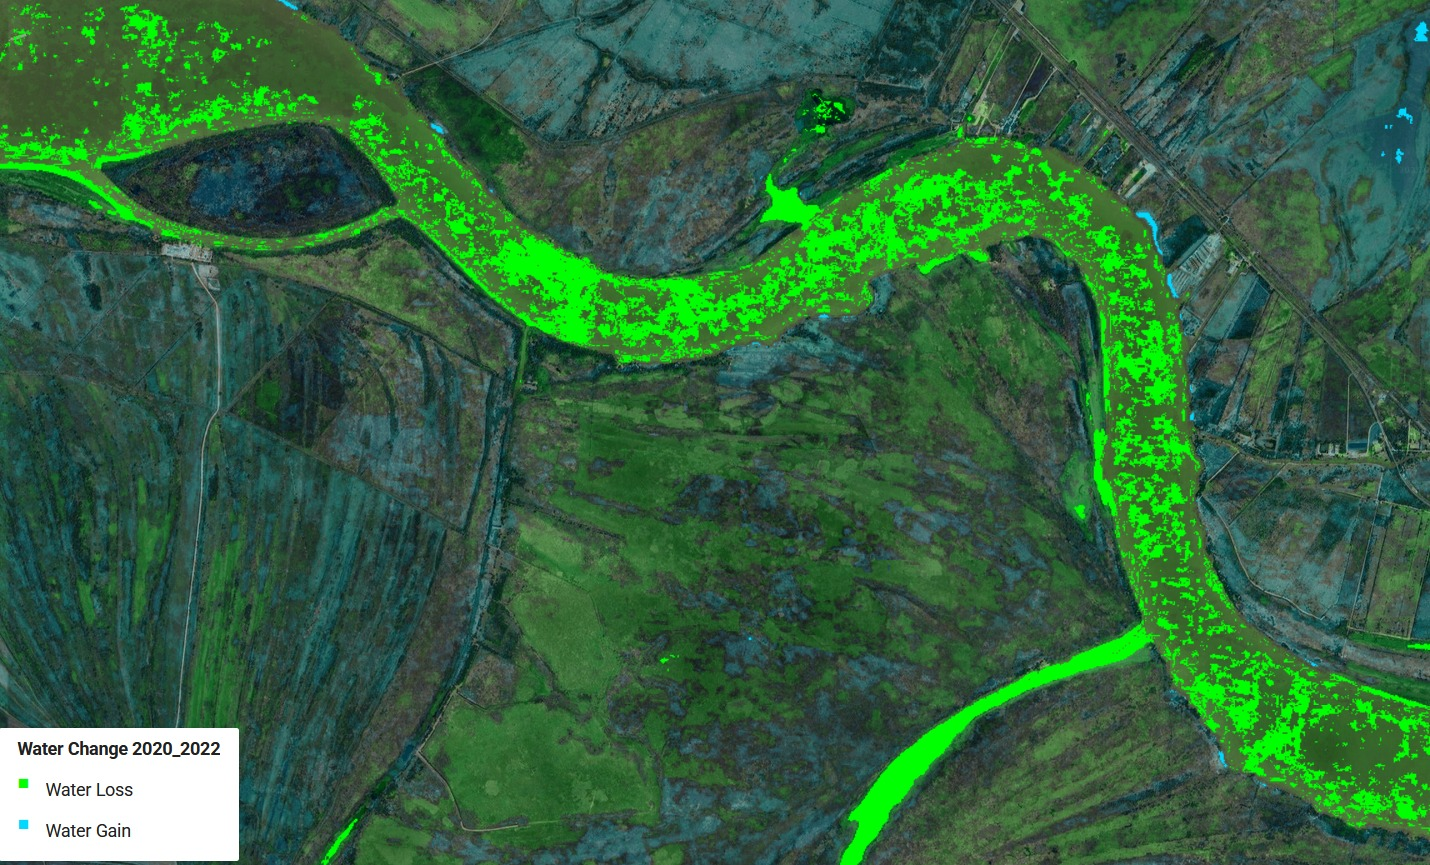
\includegraphics[width=\linewidth, height =5cm]{figures/ch5/2020-2022.jpg}
        \caption{2020-2022}
        \label{fig:second}
    \end{subfigure}
    

    % Second row of subfigures (add some vertical space)
    \vspace{0.5cm}

    % Second row of subfigures
    \begin{subfigure}[b]{0.48\textwidth}
        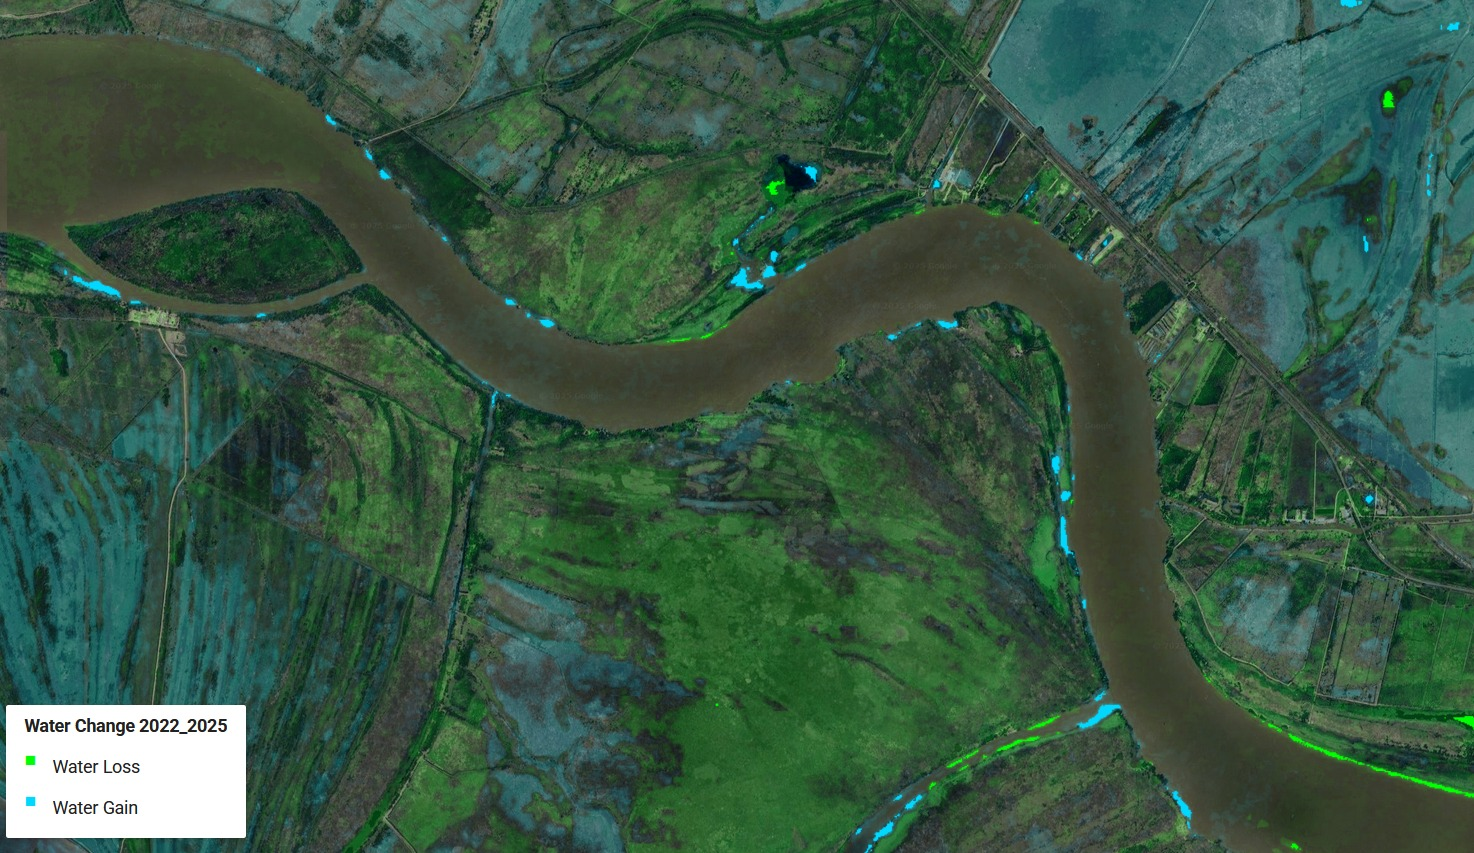
\includegraphics[width=\linewidth, height =5cm]{figures/appendix-g/2022-2025.jpg}
        \caption{2022-2025}
        \label{fig:second}
    \end{subfigure}
    \hfill
    \begin{subfigure}[b]{0.48\textwidth}
        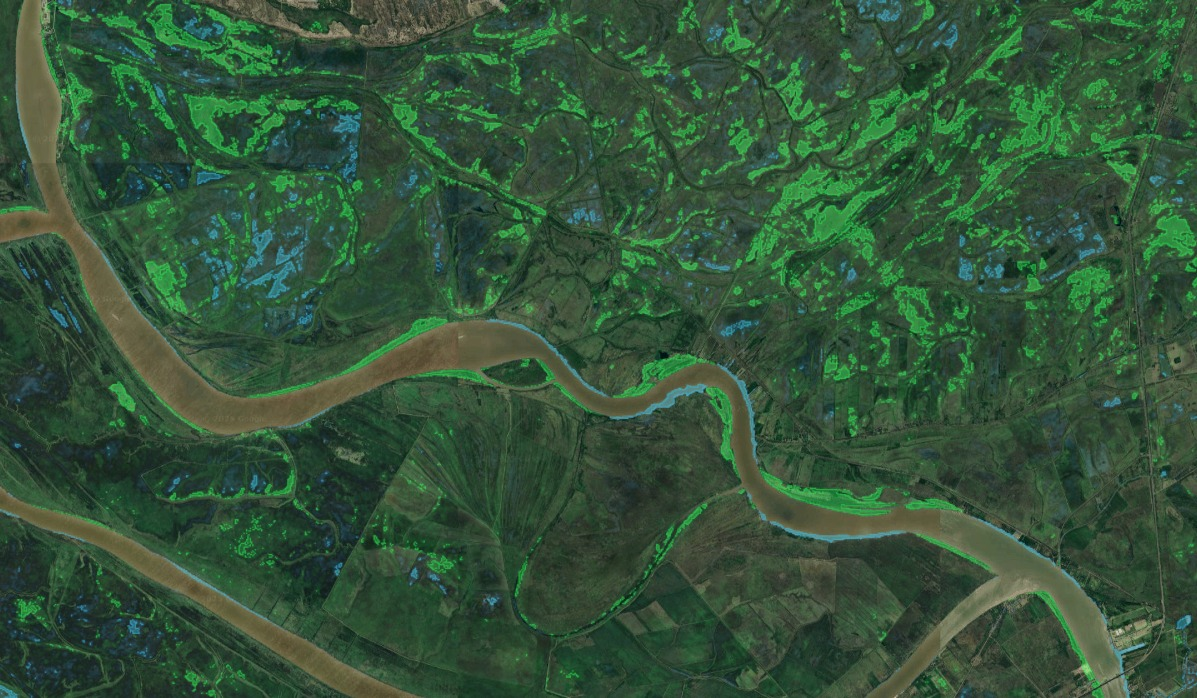
\includegraphics[width=\linewidth, height =5cm]{figures/ch4/1985-2025.jpg}
        \caption{1985-2025}
        \label{fig:second}
    \end{subfigure}

    \caption{All Changes in Water on the Area of Interest Part 2}
    \label{fig:All Changes in Water on the Area of Interest Part 2}
\end{figure}

\newpage
\section{Google Earth Engine Data}
In this part, all the maps with the possible measurements in the last years are shown, for the years 2022, 2020, 2017, 2015, 2013, 2010, 2005, 2003, and 1985.
First, the surface was recent surface was calculated based on the 2022 map on Google Earth. Then, the illustrations follow of this area of 2022 applied onto the other years data. All these images can be found below. After that, the same principle is applied for the second part of the camping which was not measured during the field trip, but seemed to be relevant based on the Google Earth study.

\subsection{Camping Surface of 2022}
The values of the perimeter and surface of the Camping in 2022 can be found in the table below. 

\begin{table}[h]
\centering
\caption{Measurements of Camping La Blanqueada in 2022}
\label{tab:Measurements of Camping La Blanqueada in 2022}
\begin{tabular}{l S[table-format=5.2] S[table-format=5.2]}
\toprule
\textbf{Location} & \textbf{Perimeter(m)} & \textbf{ Area (m²)} \\
\midrule
La Blanqueada & 1520.46 m & 88494.3 m²\\
\bottomrule
\end{tabular}
\end{table}

Next, follow the maps of how these measurements relate to the historical data of 2022-1985.
\begin{figure}[H]
    \centering
    % First row of subfigures
    \begin{subfigure}[b]{0.48\textwidth}
        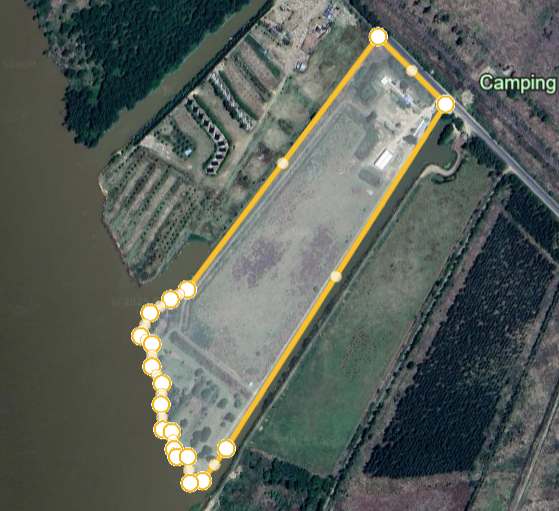
\includegraphics[width=\linewidth, height =5cm]{figures/appendix-g/opp2022.png}
        \caption{2022}
        \label{fig:second}
    \end{subfigure}
    \hfill
    \begin{subfigure}[b]{0.48\textwidth}
        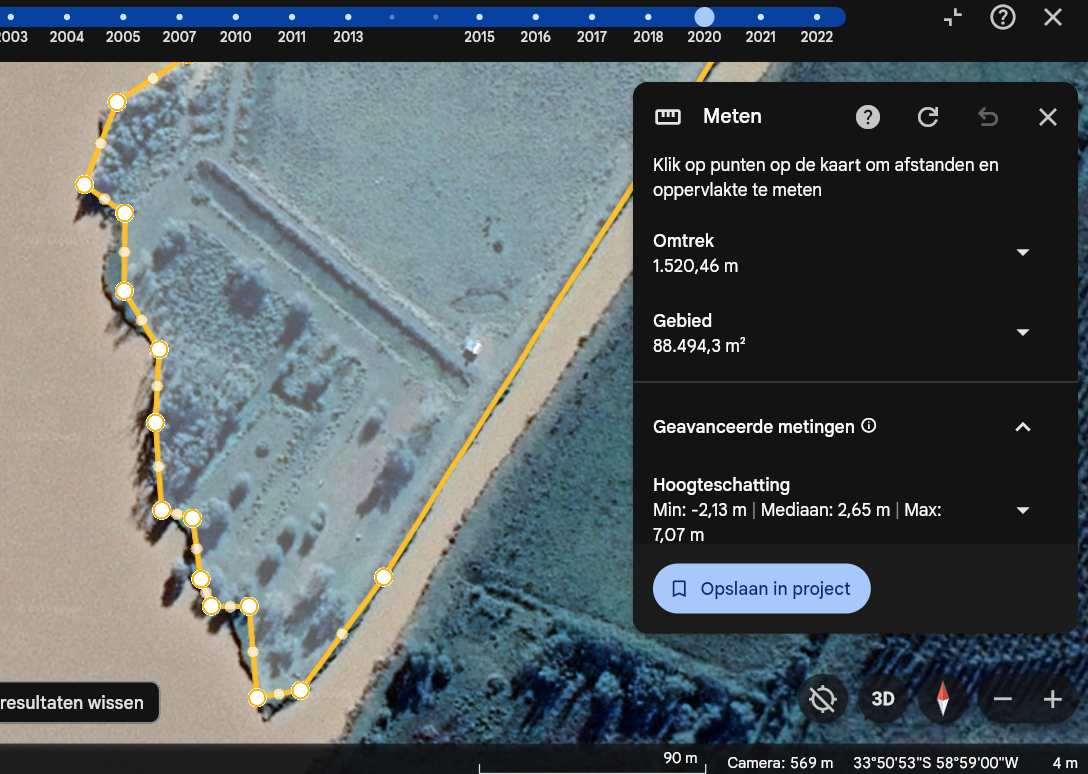
\includegraphics[width=\linewidth, height =5cm]{figures/appendix-g/opp2020.png}
        \caption{2020}
        \label{fig:second}
    \end{subfigure}
    

    % Second row of subfigures (add some vertical space)
    \vspace{0.5cm}

    % Second row of subfigures
    \begin{subfigure}[b]{0.48\textwidth}
        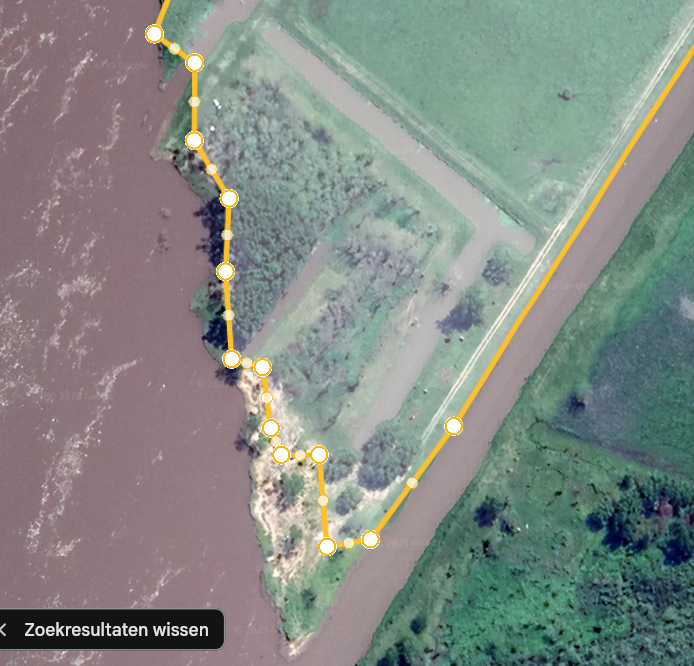
\includegraphics[width=\linewidth, height =5cm]{figures/appendix-g/opp2018.png}
        \caption{2018}
        \label{fig:second}
    \end{subfigure}
    \hfill
    \begin{subfigure}[b]{0.48\textwidth}
        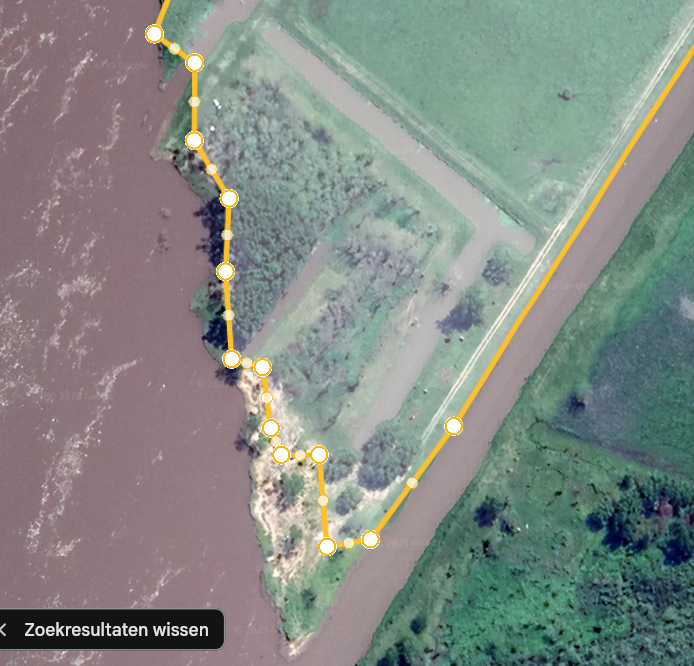
\includegraphics[width=\linewidth, height =5cm]{figures/appendix-g/opp2017.png}
        \caption{2017}
        \label{fig:second}
    \end{subfigure}

    \caption{All Changes of the Surface in Camping Part 1}
    \label{fig:All Changes of the Surface in Camping Part 1}
\end{figure}


\begin{figure}[H]
    \centering
    % First row of subfigures
    \begin{subfigure}[b]{0.48\textwidth}
        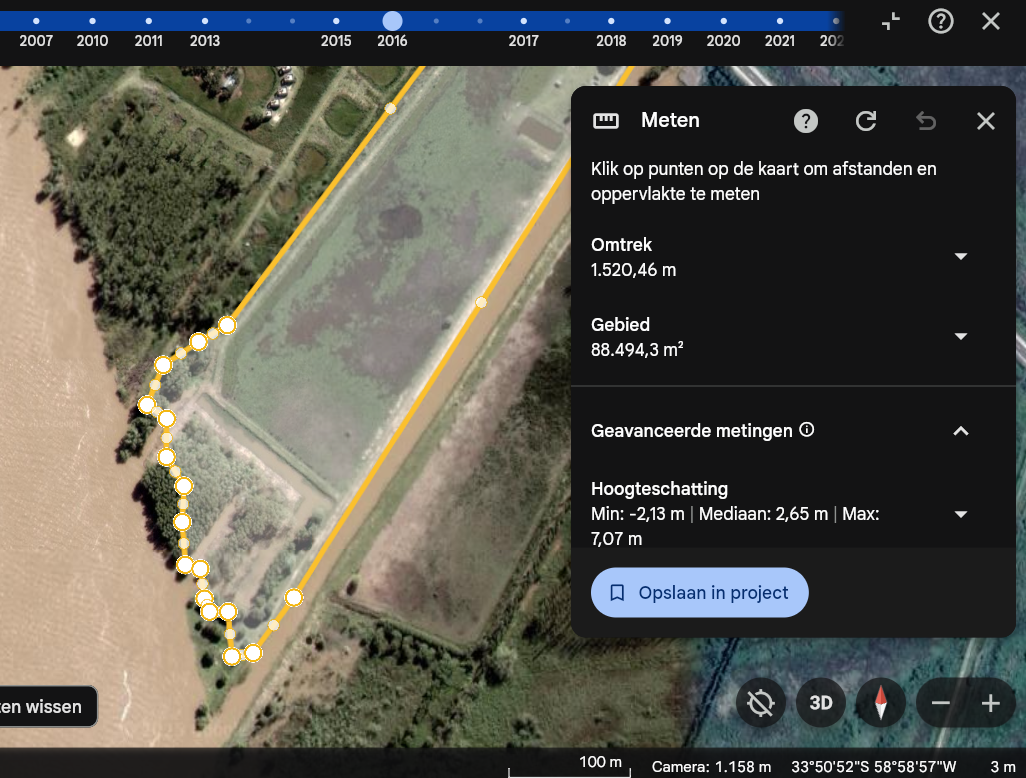
\includegraphics[width=\linewidth, height =5cm]{figures/appendix-g/opp2015.png}
        \caption{2015}
        \label{fig:second}
    \end{subfigure}
    \hfill
    \begin{subfigure}[b]{0.48\textwidth}
        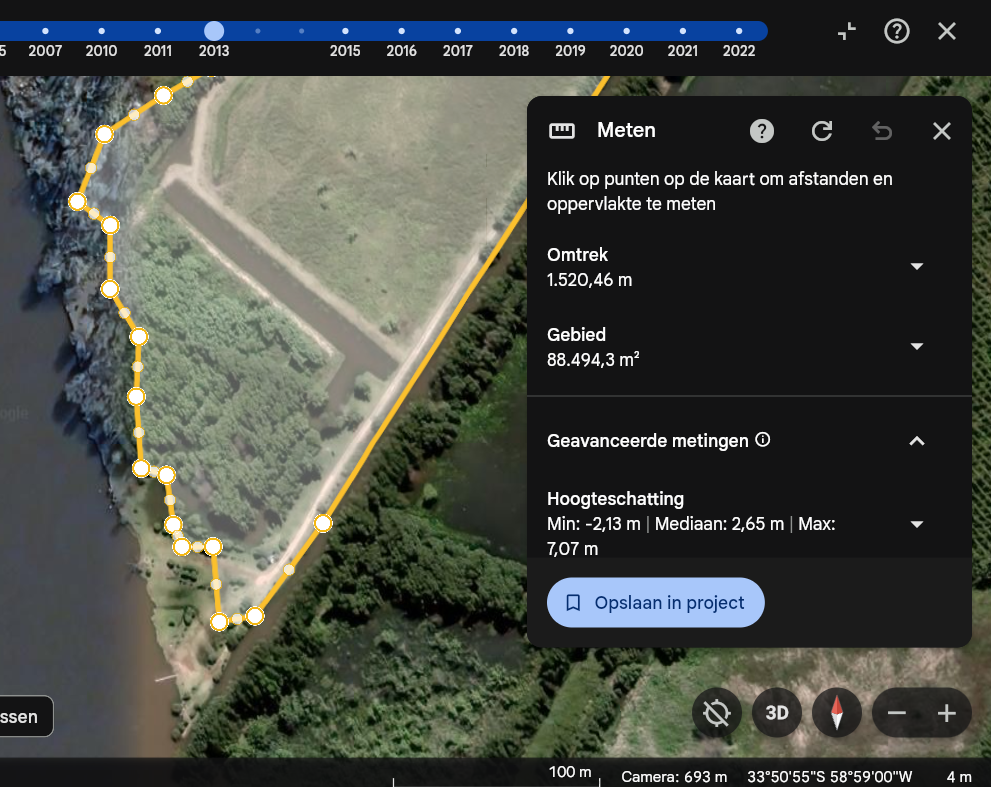
\includegraphics[width=\linewidth, height =5cm]{figures/appendix-g/opp2013.png}
        \caption{2013}
        \label{fig:a}
    \end{subfigure}
    

    % Second row of subfigures (add some vertical space)
    \vspace{0.5cm}

    % Second row of subfigures
    \begin{subfigure}[b]{0.48\textwidth}
        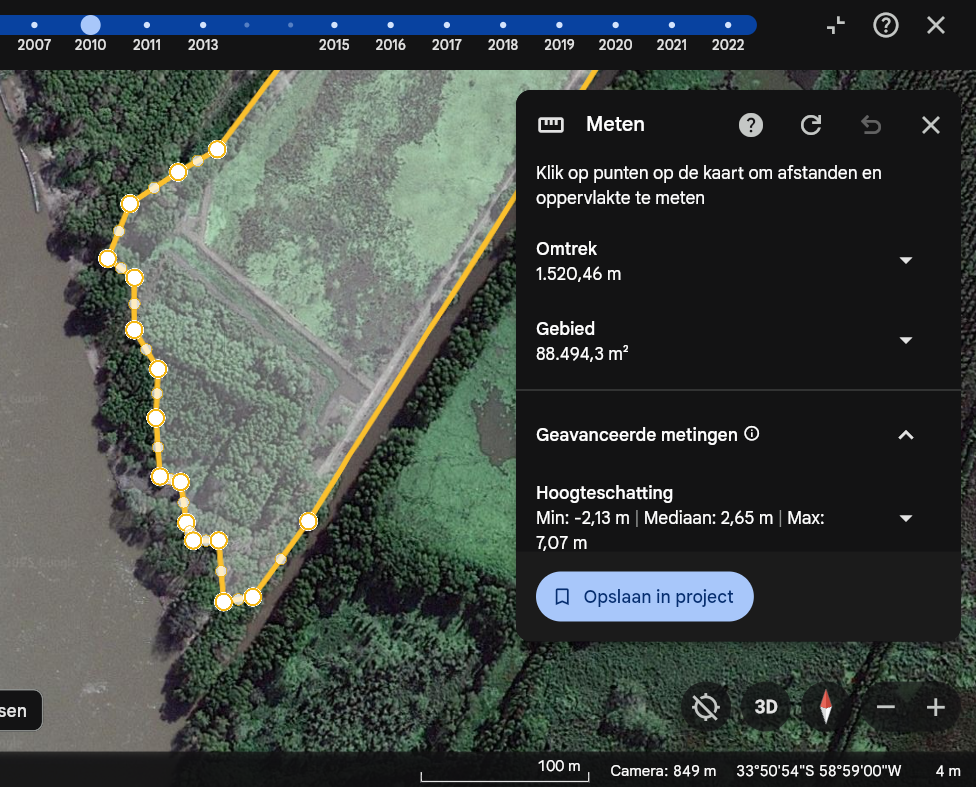
\includegraphics[width=\linewidth, height =5cm]{figures/appendix-g/opp2010.png}
        \caption{2010}
        \label{fig:second}
    \end{subfigure}
    \hfill
    \begin{subfigure}[b]{0.48\textwidth}
        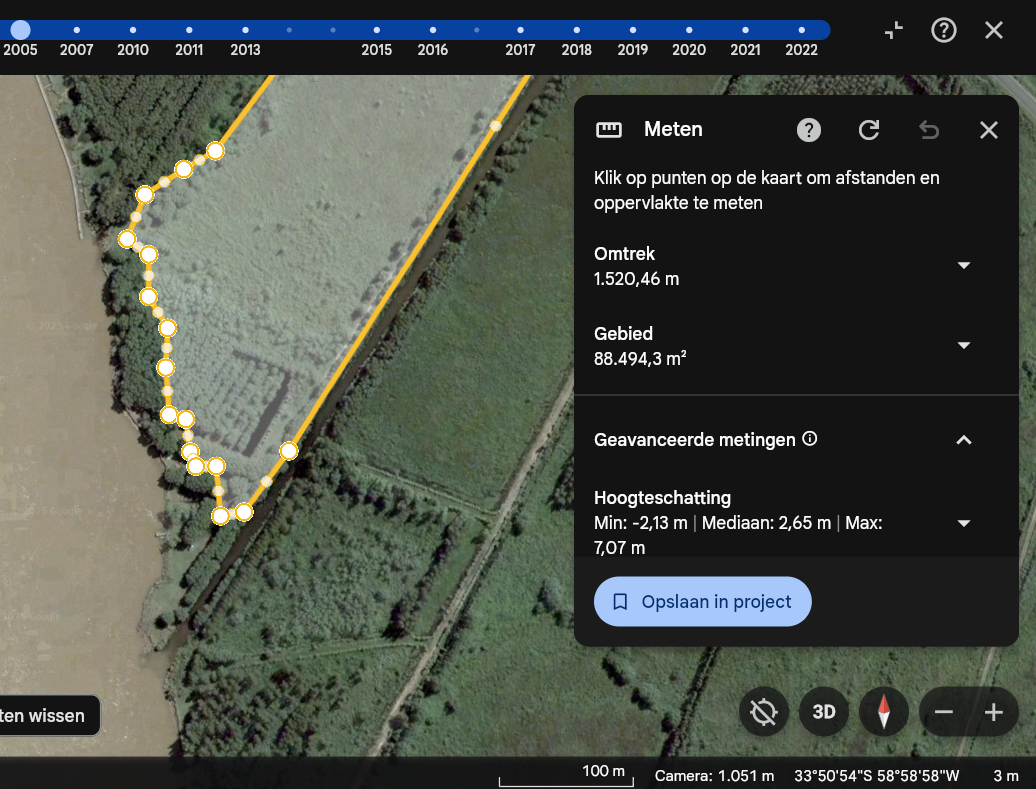
\includegraphics[width=\linewidth, height =5cm]{figures/appendix-g/opp2005.png}
        \caption{2005}
        \label{fig:second}
    \end{subfigure}

    \caption{All Changes of the Surface in Camping Part 2}
    \label{fig:All Changes of the Surface in Camping Part 2}
\end{figure}

\begin{figure}[H]
    \centering
    % First row of subfigures
    \begin{subfigure}[b]{0.48\textwidth}
        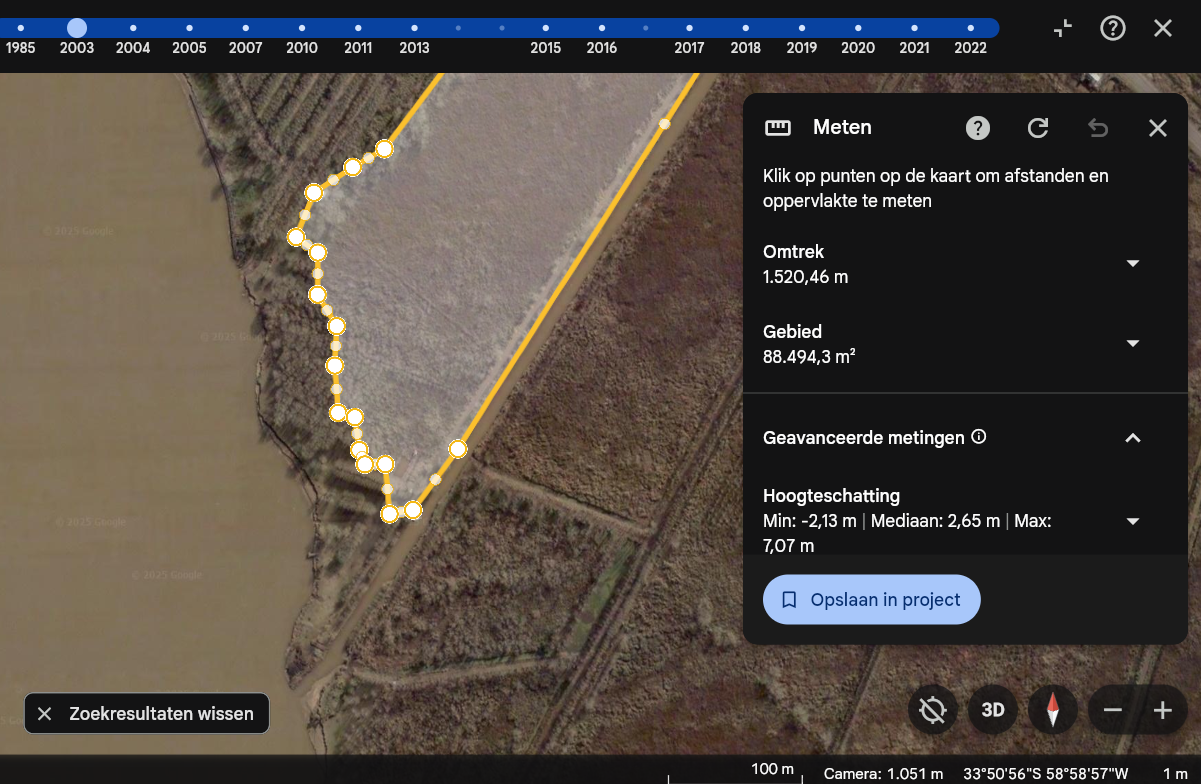
\includegraphics[width=\linewidth, height =5cm]{figures/appendix-g/opp2003.png}
        \caption{2003}
        \label{fig:second}
    \end{subfigure}
    \hfill
    \begin{subfigure}[b]{0.48\textwidth}
        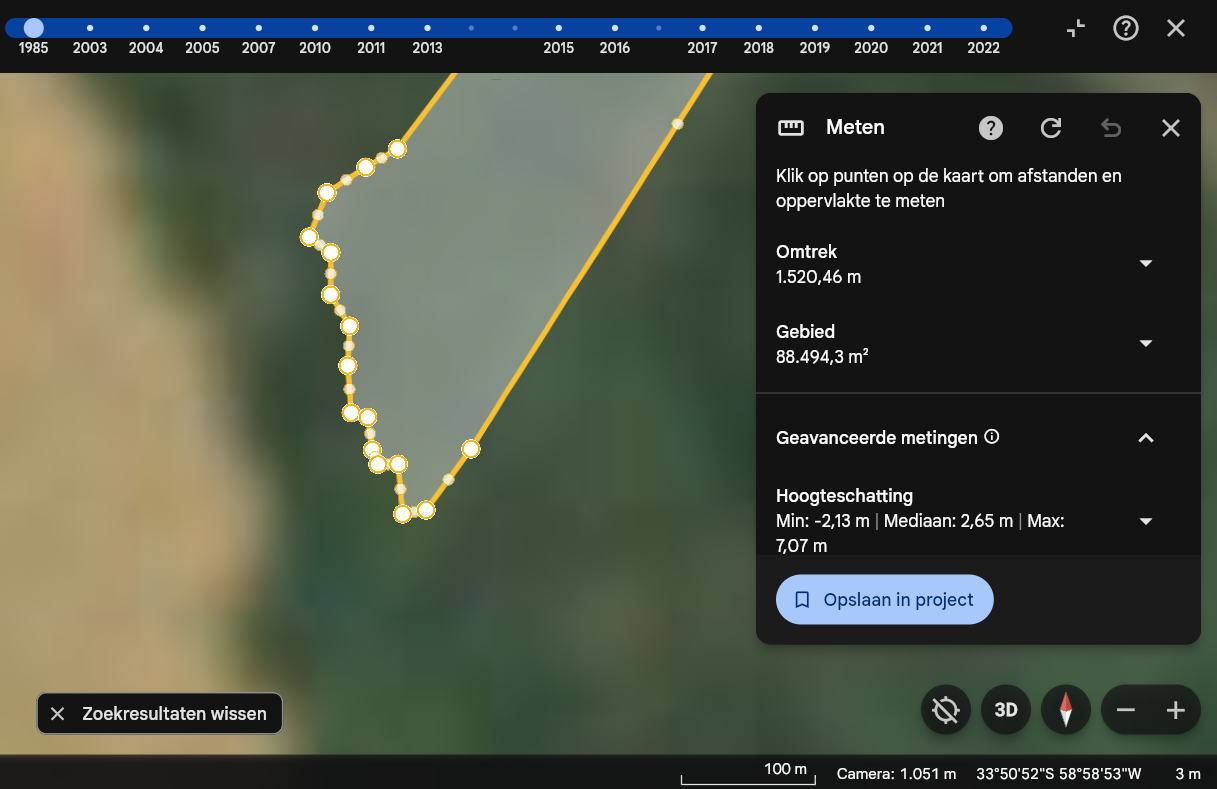
\includegraphics[width=\linewidth, height =5cm]{figures/appendix-g/opp1985.png}
        \caption{1985}
        \label{fig:second}
    \end{subfigure}
        \caption{All Changes of the Surface in Camping Part 3}
    \label{fig:All Changes of the Surface in Camping Part 3}
\end{figure} 

\subsubsection{Surface Losses Camping 2022}
Lastly, the same principle applied to the situation on the second part of the camping La Blanqueada. The values of the perimeter and surface lost compared to  2022 can be found in the table below. 

\begin{table}[h]
\centering
\caption{Surface Lost Camping La Blanqueada in 2022}
\label{tab:Surface Lost Camping La Blanqueada in 2022}
\begin{tabular}{l l l S[table-format=5.2] S[table-format=5.2]}
\toprule
\textbf{Location} & \textbf{Category} & \textbf{Colour} & \textbf{Perimeter (m)} & \textbf{Area (m²)} \\
\midrule
East Part & Actual & Yellow & 1520.46 & 88494.3 \\
East Part & Lost & Red & 786.84 & 15328.31 \\
West Part & Actual & Blue & 1203.31 & 71231.39 \\
West Part & Lost & Orange & 815.58 & 16179.99 \\
\bottomrule
\end{tabular}
\end{table}


\begin{figure}[H]
    \centering
    % First row of subfigures
    \begin{subfigure}[b]{0.48\textwidth}
        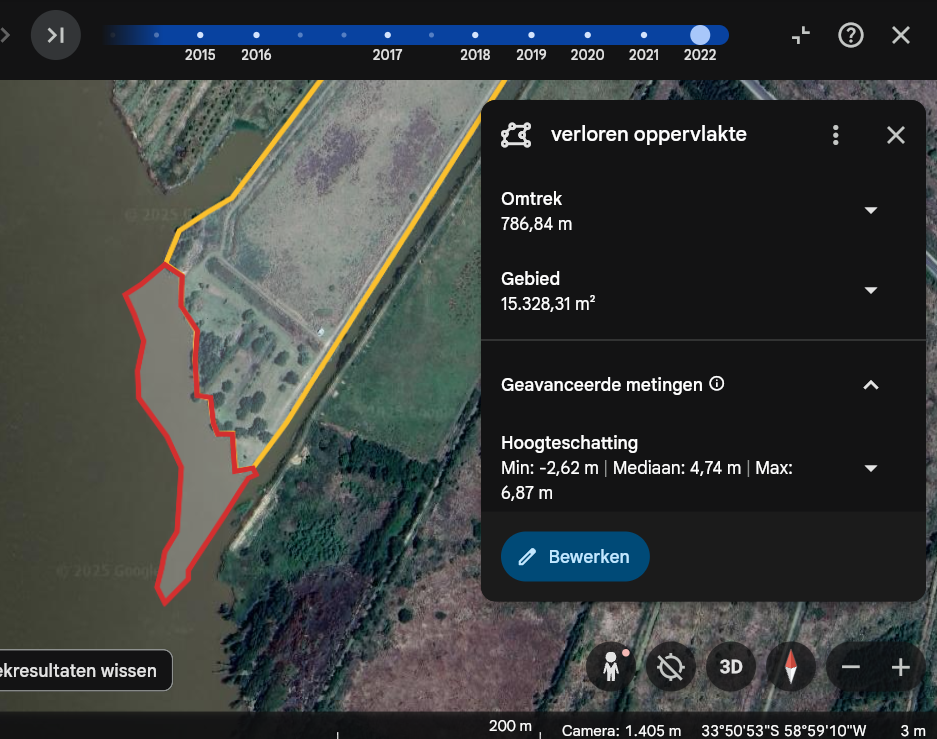
\includegraphics[width=\linewidth, height =5cm]{figures/appendix-g/verlorenopp2022.png}
        \caption{surface lost in 2022}
        \label{fig:second}
    \end{subfigure}
    \hfill
    \begin{subfigure}[b]{0.48\textwidth}
        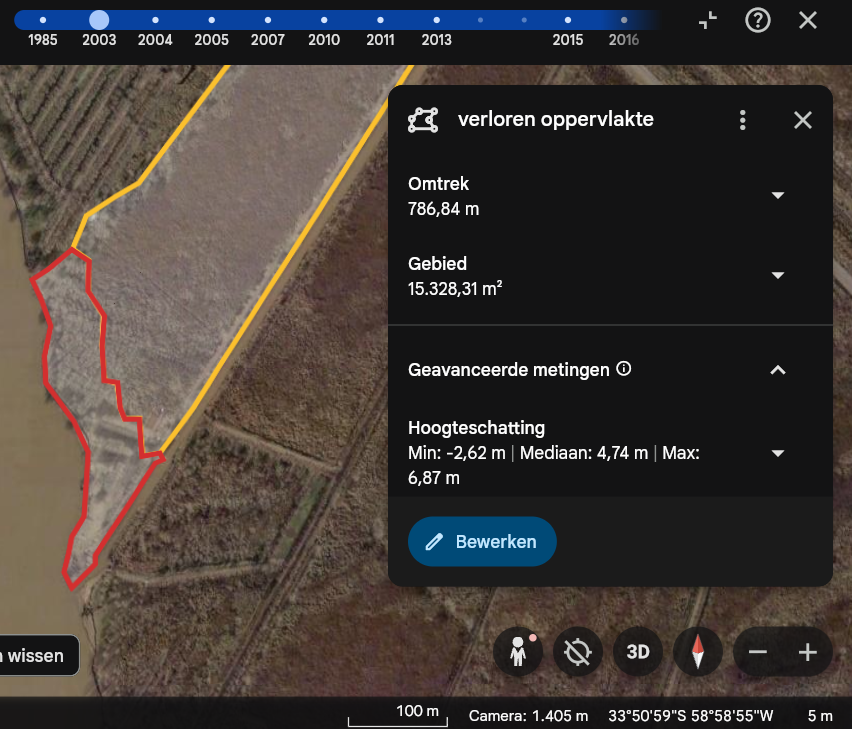
\includegraphics[width=\linewidth, height =5cm]{figures/appendix-g/verlorenopp2003.png}
        \caption{surface lost in 2003}
        \label{fig:second}
    \end{subfigure}
    

    % Second row of subfigures (add some vertical space)
    \vspace{0.5cm}

    % Second row of subfigures
    \begin{subfigure}[b]{0.48\textwidth}
        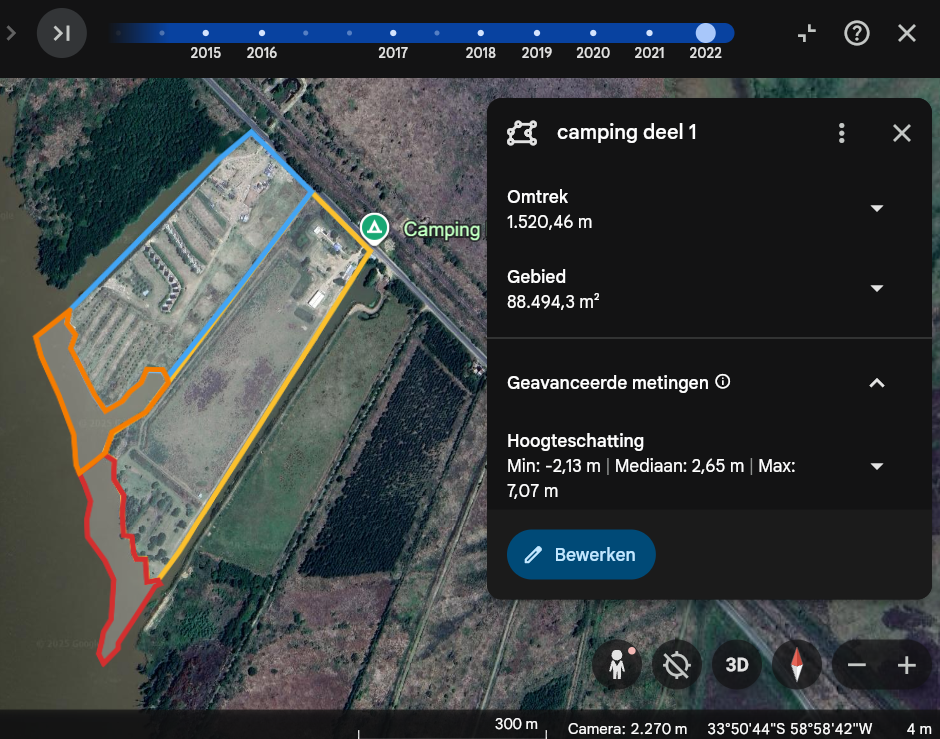
\includegraphics[width=\linewidth, height =5cm]{figures/appendix-g/delen2022.png}
        \caption{second part camping 2022}
        \label{fig:second}
    \end{subfigure}
    \hfill
    \begin{subfigure}[b]{0.48\textwidth}
        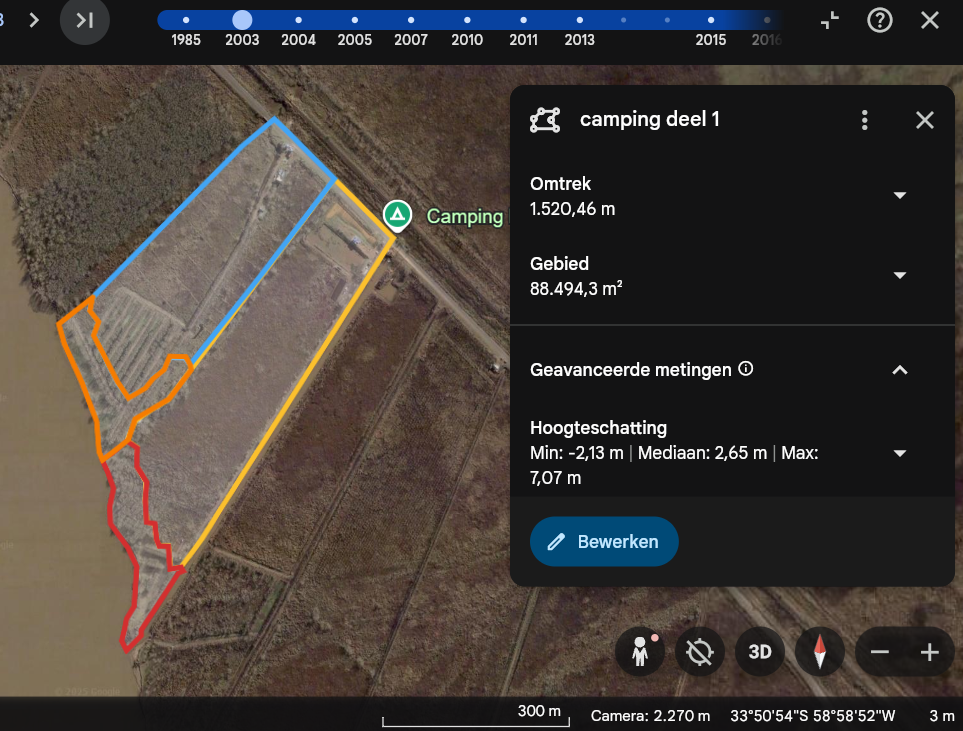
\includegraphics[width=\linewidth, height =5cm]{figures/appendix-g/delen2003.png}
        \caption{second part camping 2003}
        \label{fig:second}
    \end{subfigure}

    \caption{All Surface Losses in Camping }
    \label{fig:All Surface Losses Camping appendix}
\end{figure}

From the values in Table G.2, one can calculate the rate of change in the last 20 years or so with the help of the following formula.

$\text{Loss Ratio} = \frac{\text{Loss}}{\text{Total Surface}}$

Consequently:

$\text{Loss Ratio} = \frac{\text{Loss}}{\text{Surface in 2022 + Loss}}$

Applying this to both sides of the Camping gives:

$\text{Loss Ratio (East)} = \frac{15328.31}{88494.3 + 15328.31}$
$\frac{15328.31}{103822.61} = 0.1476$ 

$\text{Loss Ratio (West)} = \frac{16179.99}{71231.39 + 16179.99}$ 
$\frac{16179.99}{87411.38} = 0.1851 $ 

Together, these results can are found in Table G.3.

\begin{table}[h]
\centering
\caption{Loss Ratio for Camping La Blanqueada in 2022}
\label{tab:LossRatio}
\begin{tabular}{l c}
\toprule
\textbf{Location} & \textbf{Loss Ratio (\%)} \\
\midrule
East Part & 14.76 \\
West Part & 18.51 \\
\bottomrule
\end{tabular}
\end{table}

Using geometry and more measurements on Google Earth, the loss in length of the land on the shore is ranging from 45 to 132 meters in the most extreme case down south east of the camping zone, which can be seen in the Figure below. They are showed by the purple lines.

\begin{figure}[H]
    \centering
    % First row of subfigures
    \begin{subfigure}[b]{0.48\textwidth}
        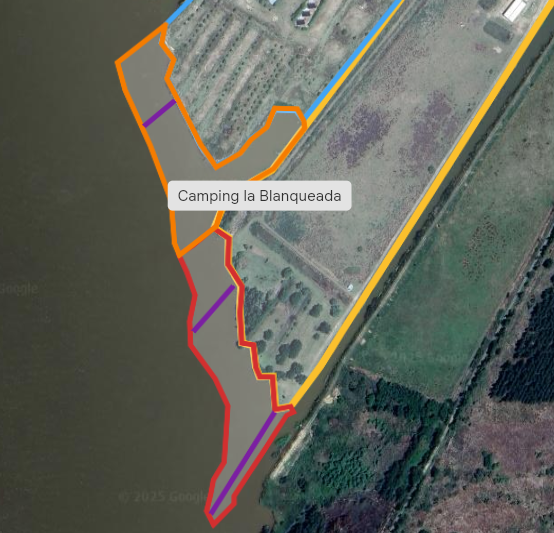
\includegraphics[width=\linewidth, height =6
        cm]{figures/appendix-g/length.png}
        \caption{Lengths of the lost land}
        \label{fig:second}
    \end{subfigure}
\end{figure}
